
%----------------------------------------------------------------------------------------
%	PACKAGES AND OTHER DOCUMENT CONFIGURATIONS
%----------------------------------------------------------------------------------------

\documentclass{article}

\usepackage{fancyhdr} % Required for custom headers
\usepackage{lastpage} % Required to determine the last page for the footer
\usepackage{extramarks} % Required for headers and footers
\usepackage{graphicx} % Required to insert images
\usepackage{mathtools, bm}
\usepackage{amssymb, bm}
\usepackage{graphicx}
\usepackage{float}

\usepackage{algorithm}
\usepackage[noend]{algpseudocode}

% Margins
\topmargin=-0.45in
\evensidemargin=0in
\oddsidemargin=0in
\textwidth=6.5in
\textheight=9.0in
\headsep=0.25in


\linespread{1.1} % Line spacing

% Set up the header and footer
\pagestyle{fancy}
\lhead{\hmwkAuthorName} % Top left header
\chead{\hmwkClass\ (\hmwkClassInstructor\ \hmwkClassTime): \hmwkTitle} % Top center header
\rhead{\firstxmark} % Top right header
\lfoot{\lastxmark} % Bottom left footer
\cfoot{} % Bottom center footer
\rfoot{Page\ \thepage\ of\ \pageref{LastPage}} % Bottom right footer
\renewcommand\headrulewidth{0.4pt} % Size of the header rule
\renewcommand\footrulewidth{0.4pt} % Size of the footer rule

\setlength\parindent{0pt} % Removes all indentation from paragraphs

%----------------------------------------------------------------------------------------
%	DOCUMENT STRUCTURE COMMANDS
%	Skip this unless you know what you're doing
%----------------------------------------------------------------------------------------

% Header and footer for when a page split occurs within a problem environment


% Header and footer for when a page split occurs between problem environments
   
%----------------------------------------------------------------------------------------
%	NAME AND CLASS SECTION
%----------------------------------------------------------------------------------------
\newcommand{\logoepfl}{
  \begin{center}
    
\includegraphics[width=4cm]{img/epfl.jpg}
  \end{center}
  \vspace{0.3cm}
  \hrule
}


\newcommand{\hmwkTitle}{Decentralized Data Sharing System based on Secure Multiparty Computation} % Assignment title
\newcommand{\hmwkDueDate}{Autumn 2017} % Due date
\newcommand{\hmwkClass}{IN, LCA1} % Course/class
\newcommand{\hmwkClassTime}{} % Class/lecture time
\newcommand{\hmwkClassInstructor}{D.Froelicher, J.Troncoso-Pastoriza} % Teacher/lecturer
\newcommand{\hmwkAuthorName}{Max Premi} % Your name

%----------------------------------------------------------------------------------------
%	TITLE PAGE
%----------------------------------------------------------------------------------------
\title{
\logoepfl
\vspace{2in}
\textmd{\textbf{\hmwkClass:\ \hmwkTitle}}\\
\normalsize\vspace{0.1in}\small{Due\ on\ \hmwkDueDate}\\
\vspace{0.1in}\large{\textit{\hmwkClassInstructor\ \hmwkClassTime}}
\author{\textbf{\hmwkAuthorName}}
\vspace{3in}
}

%----------------------------------------------------------------------------------------

\begin{document}

\maketitle

\newpage
\section*{Abstract}
\addcontentsline{toc}{section}{Abstract}
Unlynx and Prio are two privacy-preserving data sharing systems, with each its way to encode, decode and aggregate data. While Unlynx uses homomorphic encryption based on Elliptic Curve ElGamal and zero-knowledge proofs, Prio uses Secret-sharing encoding and \textit{secret-shared non-interactive proofs}(SNIP's) to validate the data, which is supposed to perform much better than classic zero-knowledge proof in term of computation time, by doing a trade-off execution time/bandwidth.\\
We consider $m$ servers that constitute the collective authority whose goal is to verifiably compute aggregation functions over data send by $n$ data providers.\\
Several problems arise when you want to compare Unlynx and Prio. First, servers are static in the first one but not in the second, and the threat model is not exactly the same, as you need to trust at least one server in Unlynx, but all in Prio for correctness. Privacy is assured if at least one server is trusted for both systems. Then for Unlynx, data providers have all their data encrypted, while Prio does not use homomorphic encryption, and do not need to store data at all. Indeed Unlynx requires the data to be stored encrypted with a collective key, whereas Prio can proceed data decomposed in shares, sent by clients directly.\\
Prio also extends classic private aggregation techniques to enable collection of different class of statistics such as least-square regression, unlike Unlynx System, that can only compute sum and count query over data.\\
The goal of this project is to, first implement Prio in the Unlynx framework, second to implement input validation for Unlynx, and then modify both protocols to run with the least significant difference in term of assumption and model.\\
Eventually, if possible, we want to design a system that implements the best of both privacy-preserving data sharing protocols. The idea would be to use Prio encoding to do more than just summing and counting in Unlynx, by removing the encryption at the data provider, and doing the computation locally and then transfer to the server in an encrypted way.\\

-------------------------------------------------
%	TABLE OF CONTENTS
%----------------------------------------------------------------------------------------

\newpage
\tableofcontents
\newpage


%----------------------------------------------------------------------------------------
%	BEGIN OF REPORT
%----------------------------------------------------------------------------------------

\section*{Introduction}
\addcontentsline{toc}{section}{Introduction}
Nowadays, tons of data are generated by us about what we do and are used to compute statistics, by different parties. Even if these statistics are collected with the goal of learning useful aggregate information about the users/population, for example, health or work statistics for a country \cite{swiss}, it might end in collecting and storing private data from data provider, which poses a serious privacy and security problem.\\
We can illustrate this example with the numerous problem of Cloud leaking that happened several times in the past years \cite{pentagon}, or the divulgation of sensitive health data such as susceptibility to contract diseases, that can be used against one individual \cite{sell}. They might even be disclosed, sold for profit \cite{sold} or be used by agencies for targeting and mass surveillance goals, as some countries have not highly regulated Data privacy law (we can take the example of the U.S \cite{law}).\\
The need to collect data and to share them in a privacy-preserving way has become crucial in this context, and lot of research has been done on this topic.\\
A lot of techniques have been developed through the years, by major technology companies such as Apple \cite{apple}, but also researcher in Universities \cite{unlynx,prio}.\\
First, systems that use "Randomize response for differential privacy" \cite{randomized} were developed. It changes a value with probability $p < 0.5$, and by summing a large number of noisy value, the aggregation is still a good estimation of the real values. This technique is well scalable and perform nicely, but assure only \textit{weak privacy}.\\
So encryption system was developed to solve this problem.
However, by gaining \textit{privacy}, these protocols sacrifice \textit{robustness} and \textit{scalability}, which are two important aspects to keep in mind while designing a decentralized system. Privacy is necessary so that no leak in the sensitive data happens, and robustness characterizes the correctness of the computation. The trade-off between both should be reasonable, as we do not want any data to be leaked, and the server has to correctly compute under given circumstances.\\
These difficulties lead to the use of legal agreements rather than technical solutions, as only a few of the systems have been deployed in the real world. This agreement is not a robust solution for several reasons.\\
One of them is centralization. Centralized systems are still widely used \cite{dyadic, centralized} because they are way simpler and use a trusted third party. But these trusted parties still are a single point of failure in the system.\\
Another reason is that data providers have begun to realize the importance and value of their own data.
This is why decentralized systems are becoming more popular, and desirable. We can also illustrate the growth of decentralized systems with the rise of Cryptocurrencies such as Bitcoin \cite{bitcoin}.\\
In this paper, we present the implementation of Prio into Unlynx, an implementation of Unlynx's input validation and a theoretical comparison and discussion for future possible new systems that combines, if possible, the best part of each paper.
	
\section*{Contributions}
\addcontentsline{toc}{section}{Contributions}
In this paper, the following contributions are made:\\
- An implementation of Prio SNIPs system in Unlynx, represented as two new protocols, and a new service. It includes the validation and the aggregation. It also contains the different data types supported by Prio.\\

- The implementation of a proof for input range validation for Elliptic Curve ElGamal, using pairing on a specific Elliptic Curve. This allows the server to exclude faulty data sent by possible malicious clients. The range to check is $[0,u^l]$ with $u,l$ taking arbitrary values.\\

- An evaluation of both this protocol in terms of privacy and efficiency, with a comparison with the most similar settings. Then a conclusion on which system suits better the needs of large-scale real-world scenario.


\section*{Background}
\addcontentsline{toc}{section}{Background}
\subsection*{Collective Authority}
Nowadays, applications and systems rely on third-party authorities to provide security service. For example the creation of certificate to prove ownership of a public key. A collective authority is a set of servers that are deployed in a decentralized and distributed way, to support a given number of protocols.\\
Each of them possesses a private-public key pair $(k_i,K_i)$, where $K_i = k_i B$ with $k_i$ is a scalar and $K_i$ a point in a given Elliptic Curve. This authority constructs a public key $K = \sum_{i=1}^{m}{K_m}$ which is the sum of all the server's public key. So to decrypt a message, each server partially decrypt a message encrypted using $K$, thus the collective authority key provides strongest link security, as no intermediate can decrypt the data without the contribution of all the servers.

\subsection*{ElGamal}
All scalar are picked in a field $\mathbb{Z}_p$.\\
For Unlynx, data are encrypted by using Elliptic Curve ElGamal, more precisely, $P$ is a public key, $x$ is a message mapped to a point and $B$ is a base point on the curve $\gamma$. The encryption is the following, with $r$ a random nonce:\\
$E_P(x) = (rB,x+rP)$. The homomorphic properties states that $\alpha E_P(x_1) + \beta E_P(x_2) = E_P(\alpha x_1+ \beta x_2)$\\
To decrypt, the owner of the private key $P = pB$ multiplies $rB$ and $p$ to get $rP$ and substract from $x + rP$.\\

\subsection*{Arithmetic Circuits}
An arithmetic circuit $C$ over a finite field $\mathbb{F}$ takes as input a vector $x = (x^{(1)},...x^{(L)}) \in \mathbb{F}^L $. It is represented as an acyclic graph with each vertex either be an \textit{input}, \textit{output} or a \textit{gate}.\\
There are only two types of gates, addition and multiplication ones, all in finite field $\mathbb{F}$.\\
A citcuit $C$ is just a mapping $\mathbb{F}^L \rightarrow \mathbb{F}$, as evaluatig is a walk thourght the circuit from inputs to outputs.

\subsection*{Beaver's MPC}
A Beaver triple is defined as follow:\\
$(a,b,c) \in \mathbb{F}^3$, chosen at random with the constraint that $a \cdot b = c$.\\
As we use it in a multiparty computation context, each server $i$ holds a share $([a]_i , [b]_i , [c]_i) \in \mathbb{F}^3$.\\
Using these shares, the goal is to multiply two number $x$ and $y$ without leaking anything about them. In Prio the goal is to multiply shares $[x]_i$ and $[y]_i$.\\
To do so the following values are computed:
$$[d]_i = [x]_i -[a]_i  \quad  ;  \quad  [e]_i = [y]_i - [b]_i$$ 
Then from this shares, each server can compute $d$ and $e$ and compute this formula:\\
$$\sigma_i = de/m + d[b]_i +e[a]_i + [c]_i$$
The sum of these shares yields:

\begin{equation}
\begin{split}
& \sum_{i} \sigma_i = \sum_{i}{(de/m +d[b]_i + e[a]_i + [c]_i)}\\
 & = de +db +ei + c\\
 & = (x-a)(y-b)+ (y-a)b + (z-b)a + c\\
 & = (x-a)y + (y-b)a + c\\
 & = xy -ab + c\\
 & = xy\\
\end{split}
\end{equation}
As $\sum_{i} \sigma_i = xy$, it implies that $\sigma_i = [xy]_i$ 

\subsection*{Affine-aggregatable encodings (AFEs) functions}
Given the fact that each data provider $i$ holds a value $x_i \in D$, and the server have an aggregation function $f : D^n \rightarrow A$, whose range is a set of aggregates $A$, an AFE gives an efficient way to encode data such that it is possible to compute the value of the aggregation function $f(x_1,...,x_n)$ given only the \textit{sum of the encodings} $x_1,....,x_n$.\\
It consist of three Algorithm (Encode, Valid, Decode) defined in a field $\mathbb{F}$ and two integers $k' \leq k$\\
\begin{itemize}
\item \textbf{Encode($x$)}: maps an input $x \in D$ to its encoding in $\mathbb{F}^k$
\item \textbf{Valid($y$)}: returns true if and only if $y$ is a valid encoding of some item in $D$
\item \textbf{Decode($\sigma$)}: $\sigma = \sum_{i=1}^{n}{Trunc_{k'}(Encode(x_i))} \in \mathbb{F}^{k'}$ is the input (Trunc takes the $k' \leq k$ components of the encoding), and it outputs the aggregation result $f(x_1,...,x_n)$.
\end{itemize}

\subsection*{Bilinear parings over Elliptic Curve}
Let $G_1$ and $G_T$ be additive group of points of an elliptic curve $G$ over a field $\mathbb{F}$ of order $n$ and with identity $O$. Then the mapping $e: G_1 \times G_1 \rightarrow G_T$ satisfies the following conditions:\\
For all $R,S \in G_1$ and $x \in \mathbb{F}$, $e(R,S)(x) = e(Rx,S) = e(R,Sx)$\\
For $B$ the base point, $e(B,B) \neq O$, and the mapping is efficiently computable.


\section{Unlynx System}
\subsection{Model}
Unlynx \cite{unlynx} is a privacy-preserving data sharing system developed by LCA1 \cite{lca} in collaboration with DeDiS \cite{dedis}.\\
It consists of a collective authority (CA) formed by a number $m$ of server $S_1,...,S_m$, and $n$ data providers $DP_1,...DP_n$ containing sensitive data, encrypted using EC ElGamal, following the key scheme describes in the \textbf{Background} Section. These DPs combined represent a distributed database that is used to answer queries made by a querier $Q$. The querier and DPs choose one server of the CA to communicate with and can change this choice at any given time.\\
\textbf{Functionality}: Unlynx should permit SQL queries of the form SELECT SUM(*)/COUNT(*) FROM DP,.... WHERE * AND/OR GROUP BY *, with any number of * clauses, but only equality ones.\\
\textbf{Privacy and Robustness}: Both are assured if at least one server is trusted, as we use the fact that it is allowed to publish ciphertext and their aggregation to show that the computation at the servers is actually correct. It leaks nothing as all data are encrypted.\\
Also, the data are never decrypted and a key switch protocol is used to sequentially change the encryption key from the CA's public one to the querier's $Q$ public one. This way, the privacy of data is ensured, as to temper the protocol, it is needed to collude with all server in the CA, which is not possible with the actual threat model.

\subsection{Threats}
\textbf{Collective authority servers} It is assumed an Anytrust model \cite{anytrust}. It does not require any particular server to be trusted or to be honest-but-curious. The moment it exists one server that is not malicious, functionality, security, and privacy are guaranteed.\\
\textbf{Data providers} are assumed to be honest-but-curious. The system does not protect against malicious DPs sending false information, but a solution will be discussed  in Section the \textbf{Input range validation for Elliptic Curve ElGamal}.\\
\textbf{Queriers} is assumed to be malicious, and can collude between themselves or with a subset of the CA servers.\\
It is also assumed that all network communication is encrypted and authenticated, by using a protocol like TLS for example.

\subsection{Pipeline and proof}
The protocol starts when a querier wants to retrieve some information about sensitive data. It sends the query to one of the servers of the CA. Upon receiving, the server broadcast this query to the other servers in the collective authority.\\
From here the data are privately and securely processed by the CA, before sending back the result to the querier, encrypted over the public key of the query. During all the steps of the protocol, the servers will never see the data in clear.\\
The pipeline is the following: Encryption, Verification Shuffle, Distributed Deterministic Tag, Collective Aggregation, Distributed Results Obfuscation, Key Switch. At the end of this pipeline, the querier get the data and can decrypt them to get the aggregate statistics he asked for, without any server seeing the data in clear, or knowing from which data provider the data are from.\\
The steps of the protocol will not be detailed in this paper, but some of them will be used for comparison with Prio and will be discussed in the \textbf{Implementation} section.
\begin{figure}[h]
\centering
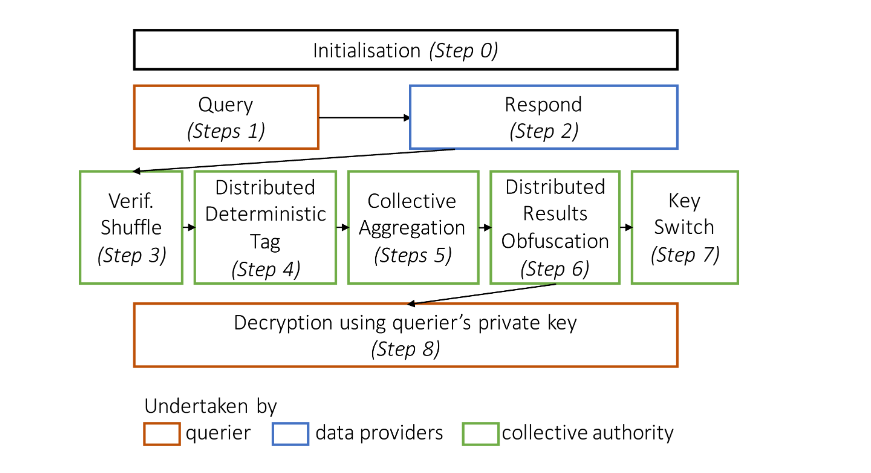
\includegraphics[scale=0.5]{img/unlynxPip.png}
\caption{Unlynx query processing pipeline}
\end{figure}
\\
\textbf{Proofs} are done thanks to zero-knowledge systems, to preserve privacy. There is one for each state of the pipeline.\\
To illustrate one of them, while doing the aggregation phase it publishes the ciphertexts and the result of their aggregation. As the data is encrypted using Elliptic curve ElGamal, it leaks nothing about the data alone.\\
However, one of the problem in Unlynx is that it exists no Input range proof for data coming from the data providers, meaning the DPs can send fraudulent data (by giving a very big number or really small) and as data are encrypted we have no way to directly check the actual value sent. This makes the whole result and computation obsolete if we assume malicious DPs, and this is why in the basic Threat model, data providers are assumed honest-but-curious. This input validation proof is implemented and described in the following section.\\

\subsection{Input range validation for Elliptic Curve ElGamal}

A problem with data's encryption is that we can not be sure if received data are correct. An example would be an aggregation where values should be in the range $[0,100)$. In the current system settings, if a malicious data provider wants to send a value of $15000$ to falsify information, it can do it. This section present an  interactive algorithm based on a classic ElGamal input range validation \cite{range}, and we will discuss its non-interactive form in the \textbf{Implementation} section.\\
We need to define some parameters before jumping into the algorithm. A scalar in the elliptic curve is defined over the field $\mathbb{Z}_p$. Also, we call $e()$ the bilinear mapping that is described in the Background section.\\
This is the algorithm that allows checking the validity of a secret $\sigma$ in a range $ [0,u^l]$. The algorithm can be adapted to check any range $[a,b]$.\\


\begin{algorithm}[H]
\caption{Interactive Range Validation}\label{euclid}
\begin{algorithmic}[1]

\State For the algorithm scalability the terms \textit{Prover} and \textit{Verifier} are used. In our case it should be clear that the prover is the data provider and the verifier the CA containing all the servers.\\
\State \textbf{Common Input:} $B$ EC base,  $P$ a public key, $ u, l$ , 2 integers and commitment $C$
\State \textbf{Prover Input:} 
$\sigma,$ the value to encode mapped to a point in the EC and $r$ a scalar in the EC such that $C = \sigma + Pr$, with $\sigma \in [0,u^l)$\\
\State  \textbf{P $\leftarrow$ V} verifiers pick $x_i \in \mathbb{Z}_p$ define $y_i \gets Bx_i$\\
send $A_{i,j} \gets B(x_i+j)^{-1}$ $ \forall j \in \mathbb{Z}_u$ and $ i \in \{0,...,m\}$\\
\State \textbf{P $\rightarrow$ V} Then prover encode the signature of the value to check in base $u$ with randomly picked $v_j$.\\
So $\forall j \in \mathbb{Z}_l $ such that $ \sigma = \sum_{j}{\sigma_j u^j}$, it picks $v_j \in \mathbb{Z}_p$ and sends $V_{i,j} = A_{i,\sigma_j}v_j$ back to server $i$\\
\State \textbf{P $\rightarrow$ V} prover pick 3 values $s_j,t_j,m_j \in \mathbb{Z}_p $, $\forall j \in \mathbb{Z}_l$ and sends to each server $i$:\\
$a_{i,j} \gets e(V_{i,j},B)(-s_j)+e(B,B)(t_j)$\\
$D \gets \sum_{j}{(u^j s_j + Pm_j)}$\\
\State \textbf{P $\leftarrow$ V} Verifier sends a random challenge $c \in \mathbb{Z}_p$\\
\State \textbf{P $\rightarrow$ V} Prover sends the following value for Verifiers to compute verification.\\
$ \forall j \in \mathbb{Z}_l$, $Z_{\sigma_j} \gets s_j-\sigma_j c$ and $Z_{v_j} \gets t_j-v_j c$\\
$Z_r = m -rc $, where $m = \sum_{j}{m_j}$\\
\State \textbf{Verifier} $i$ check that $D = Cc + PZ_r + \sum_{j}{(Bu^j Z_{\sigma_j}}) $\\
$a_{i,j} = e(V_{i,j},y)c + e(V_{i,j},B)(-Z_{\sigma_j}) + e(B,B)(Z_{v_j})$, $\forall j \in \mathbb{Z}_l$
\end{algorithmic}
\end{algorithm}

This algorithm has been adapted from the paper on Set membership over ElGamal \cite{range}, used with classic ElGamal encryption. The prover needs to compute $5l$ point multiplication in the protocol.\\
The completness follows from inspection, while soundness follows from the unforgeability of the Boneh-Boyen signature [REF].
In addition, a zero-knowledge proof must satisfy another propertie in addition to completeness and soundness. It is that if the statement is true, no verifier learns anything other than the statement is true.
This can be showed by a \textit{simulator}, that given only the statement to be proved and no access to the prover, it can produce a transcript that "look like" an interaction between a prover and the cheating verifier.\\
The simulator \textit{Sim} is constructed as follow for a verifier V:\\

\begin{algorithmic}
\State 1. \textit{Sim} retrieves $y,\{A_i\}$ from V with $i \in \mathbb{Z}_u$.
\State 2. \textit{Sim} chooses $\sigma \in [0,u^l)$, $v_j \in \mathbb{Z}_p$ and sends $V_j \gets A_{\sigma_j} v_j$, for each $\sigma_j$ such that $\sigma = \sum_{j}{\sigma_j u^j}$ with $ j \in \mathbb{Z}_l$
\State 3. \textit{Sim} chooses $s_j,t_j,m_j \in \mathbb{Z}_p$ for each $V_j$ and sends $a_j \gets e(V_j,B)(-s_j) + e(B,B)(t_j)$ for each $j$ and $D \gets $
\State 4. \textit{Sim} receives $c$ from V.
\State 5. Eventually \textit{Sim} computes for each $j$, $Z_{\sigma_j} =s_j - \sigma_j c$, $Z_{v_j} = t_j - v_j c$ and also $Z_r = m - rc$, where m is the sum of $m_j$, to V.  
\end{algorithmic}

\subsubsection*{Arbitrarty Range :}
To handle an arbitrary range $[a,b]$, it is needed to show that $\sigma \in [a,a+u^l]$ AND $ \sigma \in [b-u^l,b]$, this leads to the following formula:\\
\begin{gather*}
 \sigma \in [b-u^l,b] \Longleftrightarrow   \sigma - b + u^l \in [0,u^l) \\
\sigma \in [a,a+u^l] \Longleftrightarrow   \sigma - a  \in [0,u^l)\\
\end{gather*}
The only modification necessary in the algorithm is the verifier's check which is now:
\begin{gather*}
D = Cc+B(-B+u^l)+P(Z_r)+\sum_j{B(Z_{\sigma_j})}\\
D= Cc+B(-A)+P(Z_r)+\sum_j{B(Z_{\sigma_j})}
\end{gather*}

In the original paper, it is also discussed set membership that can be more efficient if the range is really small, for example checking that people are in the range of age [18-25] for delivering a discount.
In this case, the protocol is simpler as range validation is just a special case of set membership. The difference is that the prover sends back only one obfuscated value which is the value supposedly contained in the set.

\section{Prio System}
\subsection{Model}
Prio \cite{prio}  is also a privacy-preserving data sharing system developed at Standford University.\\
It consists of a collective authority (CA) formed by a number $m$ of server $S_1,...S_m$, and each data provider holds a private value $x_i$ that is sensitive. 
Unlike Unlynx, Prio does not encrypt private value $x_i$ that is why it's a more challenging aggregation in terms of privacy.\\
Prio is based on the splitting of each data $x$ in $m$ shares such that $\sum^m_{k=1}{x_k} = x $ in a defined a finite field $\mathbb{F}$ ie, modulo a prime $p$. This encoding helps to keep privacy, as getting $m-1$ shares doesn't leak anything about $x$ in itself.\\
Communication is assumed to be done in secure channels as previously described for Unlynx.\\
\textbf{Functionality}: Prio should permit the collective authority to compute some aggregation function $f(x_1,...x_n)$ over private values of data providers, in a way that leaks as little as possible about these, except what can be inferred from the aggregation itself.\\
It is also possible to gather more complex statistics such as variance, standard deviation, frequency count or even sets intersections/unions. All of the function quoted before is only computed from an encoding called AFE, that helps computing function with only the \textbf{sum} of the encoding. So the collective authority will always compute the sum no matter what function is asked.\\
\textbf{Privacy and Robustness}: Privacy is assured if at least one server is trusted, but robustness is satisfied if and only if all servers are trusted, as you cannot be assured that computation at the server is correct.

\subsection{Threats}
\textbf{Collective authority servers} In Prio, it is needed that one server is not malicious and trusted so that security and privacy are guaranteed.\\
Robustness against malicious server seems desirable but doing so would cost privacy and performance degradation, which is not wanted.\\
\textbf{Data providers} are assumed to be malicious. The system protects itself against malicious DPs. All data that does not pass the SNIPs proof, will be discarded.\\

\subsection{Pipeline and proof}
Pipeline is a little different than Unlynx, as first the proof is run on the data when they arrived and if it passes the proof, it is stored and aggregate later with more data.\\
First, it is needed to define an arithmetic circuit for each data provider, $Valid(.)$.
When the data provider run the circuit with its secret value as input, it output $1$, i.e $Valid(x_i)=1$.\\
This circuit is only defined in function of the number of bit of each share $[x_i]_j$ from the data provider, so it will also send a configuration file to the server so that it can reconstruct the circuit to verify the input too. From this circuit, $3$ polynomials are extracted $f,g $ and $h$.\\

The data providers first upload their shares $[x_i]_1,...,[x_i]_m$ of private value and a share of polynomial $h$ extracted from arithmetic circuit.\\
The servers verify the SNIPs provided by data providers to jointly confirm that $Valid(x_i) = 1$. If it fails, the server discards the submission.\\
Then each server saves in an accumulator the data they need to aggregate and run the collective aggregation over the verified data.\\
When received enough input, they each publish their aggregation result to yield the final aggregation ( which is the sum of all aggregation ) result.

\subsection{Prio SNIPs}
In this section, the SNIP protocol will be detailled a litlle more.\\
\textit{Assumption}: The \textbf{Valid} circuit have $M$ multiplication gates, we work over a field $\mathbb{F}$ such that $ 2M << |\mathbb{F}| $\\
\subsubsection{DP evaluation}
First the DP evaluates the circuit \textbf{Valid} on its input $x$. It construct three polynomials $f,g $ and $h$ which encode respectively the inputs wire and the ouput wire of each of the $M$ multiplication gates in the \textbf{Valid($x$)} circuit.\\
This step is done by polynomial interpolation to construct $f,g$ and get $h$ by multiplying those.\\
So polynomials $f,g$ have a degree at most $M-1$ while $h = f \cdot g$ have a degree at most $2M-2$.\\
Then the DP splits the polynomial $h$ using additive secre sharing and send the $i$th ($[h]_i$) share to server $i$
\subsubsection{Consistency checking at the server}
At this time each server $i$ holds a share $[x]_i$ and $[h]_i$ send by the data provider. From both this values, the servers can reproduce $[f]_i$ and $[g]_i$ without communicating with each other.\\
Indeed $[x]_i$ is a share of the input, and $[h]_i$ contains a share of each wire value coming out of a multiplication gate. Thus, it can derive all other values via affine operations on the wire.
\subsubsection{Polynomial identity test}
Now each server has reconstructed shares $[\hat{f}]_i, [\hat{g}]_i$ from $[h]_i$ and $[x]_i$. It holds that $ \hat{f} \cdot \hat{g} = h$ if and only if the servers collectively hold a set of wire value that, when summed is equal to the internal wire value of the \textbf{Valid($x$)} circuit computation.\\
All exeute the Schwartz-Zippel randomized polynomial identity test [REF] to check if relation holds and no data have been corrupted or malicious DPs have tried to send wrong data.\\
The principle is that if $ \hat{f} \cdot \hat{g} \neq h$, then the polinomial $ \hat{f} \cdot \hat{g} - h$ is a non-zero polynomial of degree at most $2M-2$ zeros in $\mathbb{F}$. It can have at most $2M-2$ zeros, so we choose a random $r \in \mathbb{F}$ and evaluate this polynomial, the servers will detect with probability at least $1 - \frac{2M-2}{|F|}$ that $ \hat{f} \cdot \hat{g} \neq h$.\\
The servers can use a linear operation to get share $\sigma_i = [ \hat{f}(r) \cdot \hat{g}(r) - h(r)]_i$. Then publish to ensure that $\sum_{i}{\sigma_i} = 0 \in \mathbb{F}$. If it is not $0$ the servers reject the client submission.
\subsubsection{Multiplication of shares}
Finally all servers need to multiply the shares $ [\hat{f}(r)]_i $ and $ [\hat{g}(r)]_i$ to get the share $[\hat{f}(r)]_i \cdot [\hat{g}(r)]_i$ without leaking anything to each other about the values of the two polynomials. It is here that the Beaver MPC enter the computation. Each servers also received from a trusted dealer a one-time-use shares $([a]_i,[b]_i,[c]_i) \in \mathbb{F}^3 $ such that $a \cdot b = c \in \mathbb{F}$. We can from this share, efficiently compute a multiparty multiplication of a pair secret-shared values. This only require each server to broadcast a single message.\\
The triple is generated by the data provider. The servers will be able to compute correcctly if values are corect. Moreover, even if the data provider send wrong values, the server still catch the cheating client with high probability. Indeed if $a \cdot b \neq c \in \mathbb{F}$ then we can write $a \cdot b = (c + \alpha) \in \mathbb{F}$. We can then run the polynomial identity test with $\hat{f}(r) \cdot \hat{f}(r) - h(r) + \alpha = 0$. The servers will catch a wrong input with probability at least $1 - \frac{2M-2}{|F|}$.

\subsubsection{Output verification}
If all servers are honest, each will hold a set of shares of the values if the \textbf{Valid} circuit. To confirm that \textbf{Valid($x$)} is indeed $1$ they only need to publish their share of the \textit{output wire}. Then, all server sum up to confirm that it's indeed equal to $1$, except with some small failure probability due to the polynomial identity test.


\section{Implementation}
 This section will detail what was implemented more thoroughly.
First, we will address the implementation of Prio:\\

Prio code \cite{priocode} was implemented in Go, with 3 dependencies in C (FLINT, GMP, and MPFR) to execute polynomial operations by Henry Corrigan-Gibbs.\\
This paper contribution is mostly porting code to use the multiparty computation and SNIPs in the Unlynx framework. So most of the code is used directly from the repository, but all the communication server/data provider has been reworked to be compatible with the Tree structure used in Unlynx \cite{unlynxcode}.\\
To follow the structure, the aggregation and verification protocols were split into two different protocols, even if they both work together to get the final result.\\
To be more precise, data provider send shares $[x_i]$ and $[h_i]$, servers do the SNIPs proof by evaluating the share on the \textit{Valid()} circuit, do the MPC to fuse each validation of the shares , if it passes it will aggregate the result of the SNIPs, else it will discard.\\
Let's describe the easiest protocol, the aggregation:\\
\subsubsection*{Aggregation}
The protocols are run at each server $j$, and each protocol has received a share $[x_i]_j$ from data provider $i$ represented by an array \textit{type big.Int} in Go. The protocol structure is a binary Tree.
This share actually represents the encoding in AFE of the original value which was an integer.\\

When several data have been received, aggregation start by the root protocol, that notify all children that the aggregation will start, and wait for the children to send their local sum. This notification goes down the Tree until there are no more children, and at this point each leaf $l$ aggregate locally the share by simply summing $\sum_{i}[x_i]_l$, and send the result to their unique parents. On receiving the response from its children, the other nodes aggregates locally their own shares, and send to the parent. This is done until the root as received all the data and aggregate all the data and publish them.\\
The only optimization made is the transfer of shares between server. The structure transforms these shares into a byte array and uses the method of big int to set it directly back from byte array to a big integer. This is made because the transfer functions are most efficient with bytes.\\

However, Prio has a more interesting feature that helps aggregating different type of data and doing different aggregation function. Indeed, one can represent the value to aggregate with an AFE, where the AFE will be an array of \textit{big.Int}. This helps computing OR and AND, MIN and MAX and even set intersection/union given only the aggregation of the special AFE encoding for each of this functions.\\
To illustrate an AFE, let's see the OR. To do OR($x_1,...x_n)$ where $x_i \in \{0,1\} $, $x$ is encoded as followed in $\mathbb{F}_2^{\lambda}$ (for a $\lambda$-bit string):
\begin{align*}
    Encode(x)=\left\{
                \begin{array}{ll}
                  \lambda		\text{                                          if x = 0}\\
                  \text{Random element} \in \mathbb{F}^{\lambda}_{2}		\text{											if x = 1}\\
                \end{array}
              \right.
\end{align*}
The Valid algorithm is always true as long as you have same size encoding. To Decode, we output 0 if and only if the $\lambda$-bit string is composed of $\lambda$ 0. This AFE output the boolean OR-private of the values with probability $p = 1- 2^{-\lambda}$, over the randomness of the encoding.

As seen previously, we can compute a function thanks to the sum of the AFE encoding. So the only modifications that should be made is the input data and the way the final result is computed at the root ( it's the Decode algorithm). No modification to the protocol should be made in order to compute different statistics.

\subsubsection*{Verification}
The verification protocol is the part where the multiparty computation is done. The data provider runs a function to create requests for the servers from 3 parameters: \textit{Its secret data, the number of servers, and the index of the leader for the request}.\\
This will create a request for each server, by creating a \textbf{Valid} circuit, evaluating the secret on it and constructing the polynomial. Each request contains a share of the Beaver MPC $[a]_i, [b]_i $ and $ [c]_i$, but more importantly, a share of the secret value $[x]_i$ and one of the polynomial created previously $[h]_i$.\\

The splitting is optimized by Prio, in a way that instead of picking the $s-1$ shares randomly and setting the last one, it uses a pseudo-random generator (such as AES in counter mode). You can then pick the keys and share them instead of sharing the integer directly.
Then the data provider sends to each server the request it is assigned to. From this point, before stepping into the proof, the protocol needs to initialize some parameters.\\

First, it will reconstruct the \textbf{Valid} circuit from the type and number of bits of the data provider data which is public.  Two structure called \textit{Checker} and \textit{CheckerPrecomp} implemented in the Prio code are re-used from the original implementation. They are initialized with the circuit computed previously and the leader index. The leader is the server that will return the proof result, and that coordinate the prooving protocol.
The protocol starts by assigning a request to the Checker structure and reconstituting the polynomial shares $[f]_i $ and $[g]_i$ for server $i$. It then evaluates the expression $[d]_i $ and $[e]_i$ from the MPC protocol described in a previous section. Then they all broadcast these shares, and reconstruct $d$ and $e$.
An optimization was also already done in Prio, which is verification without interpolation. The point $r$ to do the polynomial test is fixed beforehand, this way any server can interpolate and evaluate in one single step.\\
Then the goal is to check that the evaluation of $\hat{f}(r) \cdot \hat{g}(r) -\hat{h}(r) = 0$ at each server. These values are all sent to the root that checks that the sum is 0.
In the same ways as before all communication are made in bytes, and channels are used to solve waiting for result problem.\\
At the end, the protocol returns the original shares to aggregate, that is the output of the circuit evaluate on shares, if the test is true, or empty shares if the protocol fails.


\subsubsection*{Input Range}
Now we're going to look at the input range validation implementation:\\

First and foremost, pairing over elliptic curve is not supported by all the curve. So we used a pairing already implemented by DeDis in the paper dfinity repository [REF].  This is based on a Barreto-Naehrig curve implementation produced by dfinity [REF], that uses some libraries in C++ depicted in the GitHub description. We then use this curve for the whole Unlynx protocol. This is experimetal, as security should be studied again with this new parameter.\\

Then, we need to prove to a single server that a secret $\sigma$ lies in a given range. Now in a distributed service, all server of the CA should be able to check the result. For correctness, we also want that all servers participating in the computation, as there is a generation of signature from a private key, that should not be given to any DP for the soundness of the protocol. Unlike Prio, the threat model cites that no server need to be trusted or honest-but-curious, but there must exist one server that is not malicious.\\
We cannot make the computation of the key with a sequential protocol, as they will all have the same private key and if one divulgates it, the soundness of the protocol does not hold. \\

So the difficulty resides in the fact that we should compute signature in a private way, without revealing a unique collective private key to the server. So each server will have a private key, and from this point, two choices can be made. The first one is the computation of signature in a sequential way (in the same way as the key switch protocol does), and have a final public key and the same signature for each server. The second one is that each server has its own signature and does the proof, the protocol passes if and only if all server found that the secret $\sigma$ indeed lies in the given range.\\
Because of the uncertainty of the sequential creation of the Boneh signature and the resources it would need to prove correctness, the second approach was chosen.
\begin{algorithm}[H]
\caption{Non-Interactive Range Validation}\label{euclid}
\begin{algorithmic}[1]
\State \textbf{Common Input:} $B$ the base point in the EC, $P$ the public key used to encode data, $u, l$ 2 integers and commitment $C$.
\State \textbf{Prover Input:} $\sigma$ the secret integer mapped to a point and $r$ a scalar in the EC such that $C = \sigma + Pr$, $\sigma \in [0,u^l)$\\

\State \textbf{Initialization Phase}: Each server $i$ in the collective authority compute the following values :\\
Pick a random $x_i \in \mathbb{Z}_p$\\
$y_i \gets Bx_i$\\
$A_{i,j} \gets B(x_i + j)^{-1} $, $\forall i \in \mathbb{Z}_u$ and $j \in \{1,...,m\}$\\
\State  \textbf{Servers} make their signature public as well as the key $y_i$. When a query is issued by a querier $Q$, we now assume that the range are contained in the query and broadcasted by the server as usual to the data provider.\\

\State \textbf{Online Phase}: Data provider encodes the signature of the value to check in base $u$ with randomly picked $v_j$.\\
So $\forall j \in \mathbb{Z}_l $ such that $ \sigma = \sum_{j}{\sigma_j u^j}$, it picks $v_j \in \mathbb{Z}_p$ and compute $V_{i,j} = A_{i,\sigma_j}v_j$\\
It also picks 3 values $s_j,t_j,m_j \in \mathbb{Z}_p $, $\forall j \in \mathbb{Z}_l$ and sends:\\
First : a value $c = H(B,C,y_i)$, where $H()$ is a cryptographic hash function.\\  Then: $Z_r = m-rc$ and $D \gets \sum_{j}{(u^j s_j + Pm_j)}$\\
And eventually $ \forall j \in \mathbb{Z}_l$\\
$a_{i,j} \gets e(V_{i,j},B)(-s_j)+e(B,B)(t_j)$\\ $Z_{\sigma_j} \gets s_j-\sigma_j c$ and $Z_{v_j} \gets t_j-v_j c$\\
To be more precise the data provider sends the following values to ALL servers: $ c, Z_r, Z_{v_j}, Z_{\sigma_j}$ with $C$ the encrypted value public, and $D, a_{i,j}$ value published to check proof.\\

\State Server $i$ checks that $D = Cc + PZ_r + \sum_{j}{(u^j Z_{\sigma_j}}) $\\
$a_{i,j} = e(V_{i,j},y)c + e(V_{i,j},B)(-Z_{\sigma_j}) + e(B,B)(Z_{v_j})$, $\forall j \in \mathbb{Z}_l$ , and publish the result.\\

Then the server responsible for the data provider keep the value if all the published value match the one computed by the data provider.
\end{algorithmic}
\end{algorithm}

At the end of the protocol, all values computed are made public so that anyone can verify that the servers have computed the verification correctly and act accordingly.\\

The completness follows from inspection. The soundness is still based on the Boneh signature.\\
The zero-knowledge was the satisfied in the interactive version of this protocol. As we use the Fiat-Shamir heuristic [REF] to transform the protocol into a  non-interactive one, the zero-knowledge property is still assumed to hold.\\

Let's now look at the communication complexity.
The signature and public key sending are not counted as a part of the protocol, as it can be reused.\\
The prover sends $l$ blinded values $V_j$ to each verifier, as well as $l$ $Z_{\sigma_j}$ and $Z_{v_j}$, a challenge $c$
\subsubsection*{Optimizations}
The input range implementation can be furthered optimized and we will discuss the possible improvements in this sub-section as well as what was implemented in the actual framework.\\
First of all, the service implemented consists of 3 steps: Range verification, Aggregation, and Key switch. This is the best approximation of service to compare with the Prio verification and aggregation, with the least differences.\\
This service is in no case optimized, it serves as a comparison, so a lot of values are hardcoded such as the number of client submission to wait for before aggregation or the keys for encryption are chosen beforehand randomly.\\

One thing is that each server received a different structure containing all parameters to validate including $C, c, \{V\}, \{Z_v\} ,\{ Z_{\sigma}\}, D $ and $a$. We could improve the protocol to compute only once the $D$ and $Z_r$, and pick for a single value the same $m_j, t_j$ and $s_j$ at prover.\\
This would lead to a small reduction in computation time in prover side, and some bandwidth reduction for servers.

\section{Performance evaluation}

NEED TO COMPUTE THE DIFFERENT RESULTS.

\begin{itemize}


\item Scaling with number of server
\item Scaling with number of client
\item Scaling with fairly high number of both 
\item Time and Bandwidth dilemna

\end{itemize}


\section{Comparison Theory and Performance}
As explained previously, the service implemented for Unlynx range proof consists of 3 steps: Range verification, Aggregation, and Key switch. This is the best approximation of service to compare with the Prio verification and aggregation, with the least significant differences.\\
The key switch used is not the optimal one as it does not use the byte structure to communicate, due to a problem on the new Elliptic curve used.\\

The threat models are almost the same (the small difference is still in the collective authority, where the one for Unlynx is more relaxed) and we study the time it takes for an aggregation.\\
To be more precise in Prio, we measure the time, for different clients, it takes to verify all submissions, aggregate and publish the computed aggregate function.
While in Unlynx, the measured time is the sum of the verification, the aggregation of cipher and the key switch, as you need to turn back the aggregate data to readable data for the querier. 

\section{Future Work}
Depends on RESULT.

\newpage
\section*{Conclusion}
\addcontentsline{toc}{section}{Conclusion}
iufznfiozfoezizefez fze
fezfezfezfezfezfezf
ezfezfezfzefezfezfezfezfezfzefzefezfezfezfezfezfezfezfz

\newpage
\begin{thebibliography}{9}

\bibitem{unlynx} 
David Froelicher, Patricia Egger, João Sa Sousa, Jean Louis Raisaro, Zhicong Huang, Christian Mouchet, Bryan Ford and Jean-Pierre Hubaux.\\
\textit{UnLynx:} A Decentralized System for Privacy-Conscious Data Sharing. 
\textit{EPFL}
 
\bibitem{prio} 
Henry Corrigan-Gibbs and Dan Boneh.\\
\textit{Prio}: Private, Robust, and Scalable Computation of Aggregate Statistics.
\textit{Standford University}


\bibitem{range} 
Jan Camenisch, Rafik Chaabouni, and abhi shelat\\
Efficient Protocols for Set Membership and Range Proofs.
\textit{IBM Research, EPFL, U. of Virginia}

\bibitem{expose}
Keller,J., Lai,K.R., and Pelroth, N\\
How many times has your personal information been exposed to hackers ?
\\\texttt{http://www.nytimes.com/interactives/2015/07/29technology/personaltech/what-parts-of-your-information-have-been-exposed-to-hackers-quiz.html}

\bibitem{pentagon}
Classified Pentagon data leaked on the public cloud, BBC news
\\\texttt{http://www.bbc.com/news/technology-42166004}

\bibitem{apple}
Greenberg, A.\\
Apple's 'differential privacy' is about colleccting your data- but not your data.
\\\texttt{https://www.wired.com/2016/06/apples-differential-privacy-collection-data/}

\bibitem{swiss}
Departement federal de l'economie, de la formation et de la recherche DEFR.
\\\texttt{https://www.amstat.ch}

\bibitem{lca}
LCA1 laboratory, EPFL.
\\\texttt{http://lca.epfl.ch/}

\bibitem{dedis}
DeDis laboratory, EPFL.
\\\texttt{https://dedis.epfl.ch/}

\bibitem{randomized}
Warner, S. L.\\
Randomized response: A survey technique for eliminating evasive bias.\\
\textit{Journal of the American Statistical Association 60,309 (1965),63-69}

\bibitem{sold}
Smith, B.\\
Uber executive suggest digging up dirt on journalits.
\\\texttt{http://www.buzzfeed.com/bensmith/uber-executive-suggests-digging-up-dirt-on-journalists}

\bibitem{dyadic}
Dyadic security \texttt{https://www.dyadicsec.com/}

\bibitem{centralized}
Dan Bogdanov, Sven Laur, and Jan Wilemson.\\
\textit{Sharemind}: A framework for fast privacy-preserving computations. In \textit{European Symposium on Research in Computer Security}

\bibitem{anytrust}
David I Wolinsky, Hery Corrigan-Gibbs, Bryan Ford, and Aaron Jonhson.\\
Scalable anonymous group communication in the anytrust model. In \textit{5th European Workshop on System Security. 2012}


\bibitem{priocode}
Prototype implementation of Prio in Go
\\\texttt{https://github.com/henrycg/prio}

\bibitem{unlynxcode}
Decentralized privacy-preserving data sharing tool : Unlynx\\
\texttt{https://github.com/lca1/unlynx}

\bibitem{sell}
The business of Data selling\\
\texttt{https://www.theguardian.com/technology/2017/jan/10/medical-data-multibillion-dollar-business-report-warns}

\bibitem{law}
Law on Data protection in the United-States\\
\texttt{https://content.next.westlaw.com/Document/I02064fbd1cb611e38578f7ccc38dcbee/View/FullText.html?contextData=(sc.Default)\& transitionType=Default\& firstPage=true\& bhcp=1}


\bibitem{bitcoin}
Bitcoin: A Peer-to-Peer Electronic Cash System.\\
\texttt{https://bitcoin.org/bitcoin.pdf}



\end{thebibliography}


\end{document}
